\subsection{Performance Evaluation}
\label{sec:evaluation}
%\textcolor{red}{Three machines connected in an isolated 1Gbps LAN,
%    build the experimental SSO environment.
%The CPUs are Intel Core i7-4770 3.4 GHz for the IdP,
%    Intel Core i7-4770S 3.1 GHz for the RP, and Intel Core i5-4210H 2.9 GHz for users.
%Each machine is configured with 8 GB RAM and
%    installs Windows 10 as the operating system.
%The user agent is Chrome v75.0.3770.100.}

%RP(不包括特定方案的SDK)大约需要230行JAVA代码
%OIDC(MITREid)的SDK需要大约20行的JAVA代码,需要额外添加一个HTML文件(包含大约20行JavaScript代码)
%UPPRESSO的SDK需要大约1100行代码,不需要添加额外的HTML文件
%OIDC和UPPRESSO的SDK只需要RP提供两个网络接口(网址),然后在对应的网络接口中引用对应的API(每个接口对应一个API,分别命名为tokenRequestGenerate和userAccountAchieve),其他的处理流程均由SDK完成
%SPRESSO由于结构与OIDC完全不同,所以使用了SPRESSO提供的RP的开源代码
%For better evaluation, we build one RP for both UPPRESSO and MITREid Connect which is also implemented  based on Spring Boot framework, as well as the identity token transmission from user to RP in MITREid Connect is implemented by JavaScript running in RP's web page. The IdP in MITREid Connect is achieved from GitHub \cite{MITREid}. However, the SPRESSO system is downloaded from \cite{spressome} containing IdP, RP, and FWD.

\noindent {\bf Experiment setting.}
%SPRESSO encrypts the RP's domain in identity tokens and keeps the AES symmetric key known only to the RP and the user.
Of all solutions, the IdP and RP servers were deployed on Alibaba Cloud Elastic Compute Service, each of which ran Windows 10 with 8 vCPUs and 32GB RAM.
The extra forwarder server of SPRESSO ran Ubuntu 20 with 16 vCPUs, % + 16GB RAM,
 also on the cloud platform, helping to forward identity tokens to RP servers.

We conducted experiments in two settings: (\emph{a}) a browser, Chrome 104.0.5112.81, ran on a virtual machine on the cloud platform with 8 vCPUs and 32 GB memory, and (\emph{b}) the browser running locally on a PC with Core i7-8700 CPU and 32 GB memory, remotely accessed the servers.
All entities except the local browser,
were deployed in the same virtual private cloud and connected to one vSwitch, which minimized the impact of network delays.
%In both settings, the IdP server never directly communicated with RPs.

\noindent {\bf Comparisons.} We split the login flow into three phases for detailed comparisons: (1)
{\em identity-token requesting} (Step 1 in Figure \ref{fig:process}), to construct an identity-token request and send it to the IdP server; (2) {\em identity-token generation} (Step 2 of UPPRESSO), to generate an identity token at the IdP server, while the user authentication and the user-attribute authorization are excluded; and (3) {\em identity-token acceptance} (Step 3), where the RP receives, verifies, and parses the identity token.

In the identity-token requesting phase of UPPRESSO a browser downloads the two scripts,
    as described in Section \ref{sec:web-design}.
As mentioned in Section \ref{subsec:OIDC},
 to process the token retrieved from the IdP, %which is carried with a URL following the fragment identifier \texttt{\#} instead of \texttt{?} due to security considerations \cite{de2014oauth},
    in MITREid Connect and SPRESSO a user-r script is downloaded during the phase of token generation.
SPRESSO needs another script from the forwarder server in the token acceptance phase \cite{SPRESSO}.

We compared the average time required for an SSO login in three schemes based on 1,000 measurements. As shown in Figure \ref{fig:evaluation},
MITREid Connect, UPPRESSO, and SPRESSO require (\emph{a}) 63 ms, 179 ms, and 190 ms, respectively when all entities were deployed on the cloud platform,
 or (\emph{b}) 312 ms, 471 ms, and 510 ms, respectively when the user browser ran locally to visit the cloud servers.

\begin{figure}[tb]
  \centering
	\subfigure[In a virtual private cloud]{
  		\begin{minipage}[b]{0.45\textwidth}
			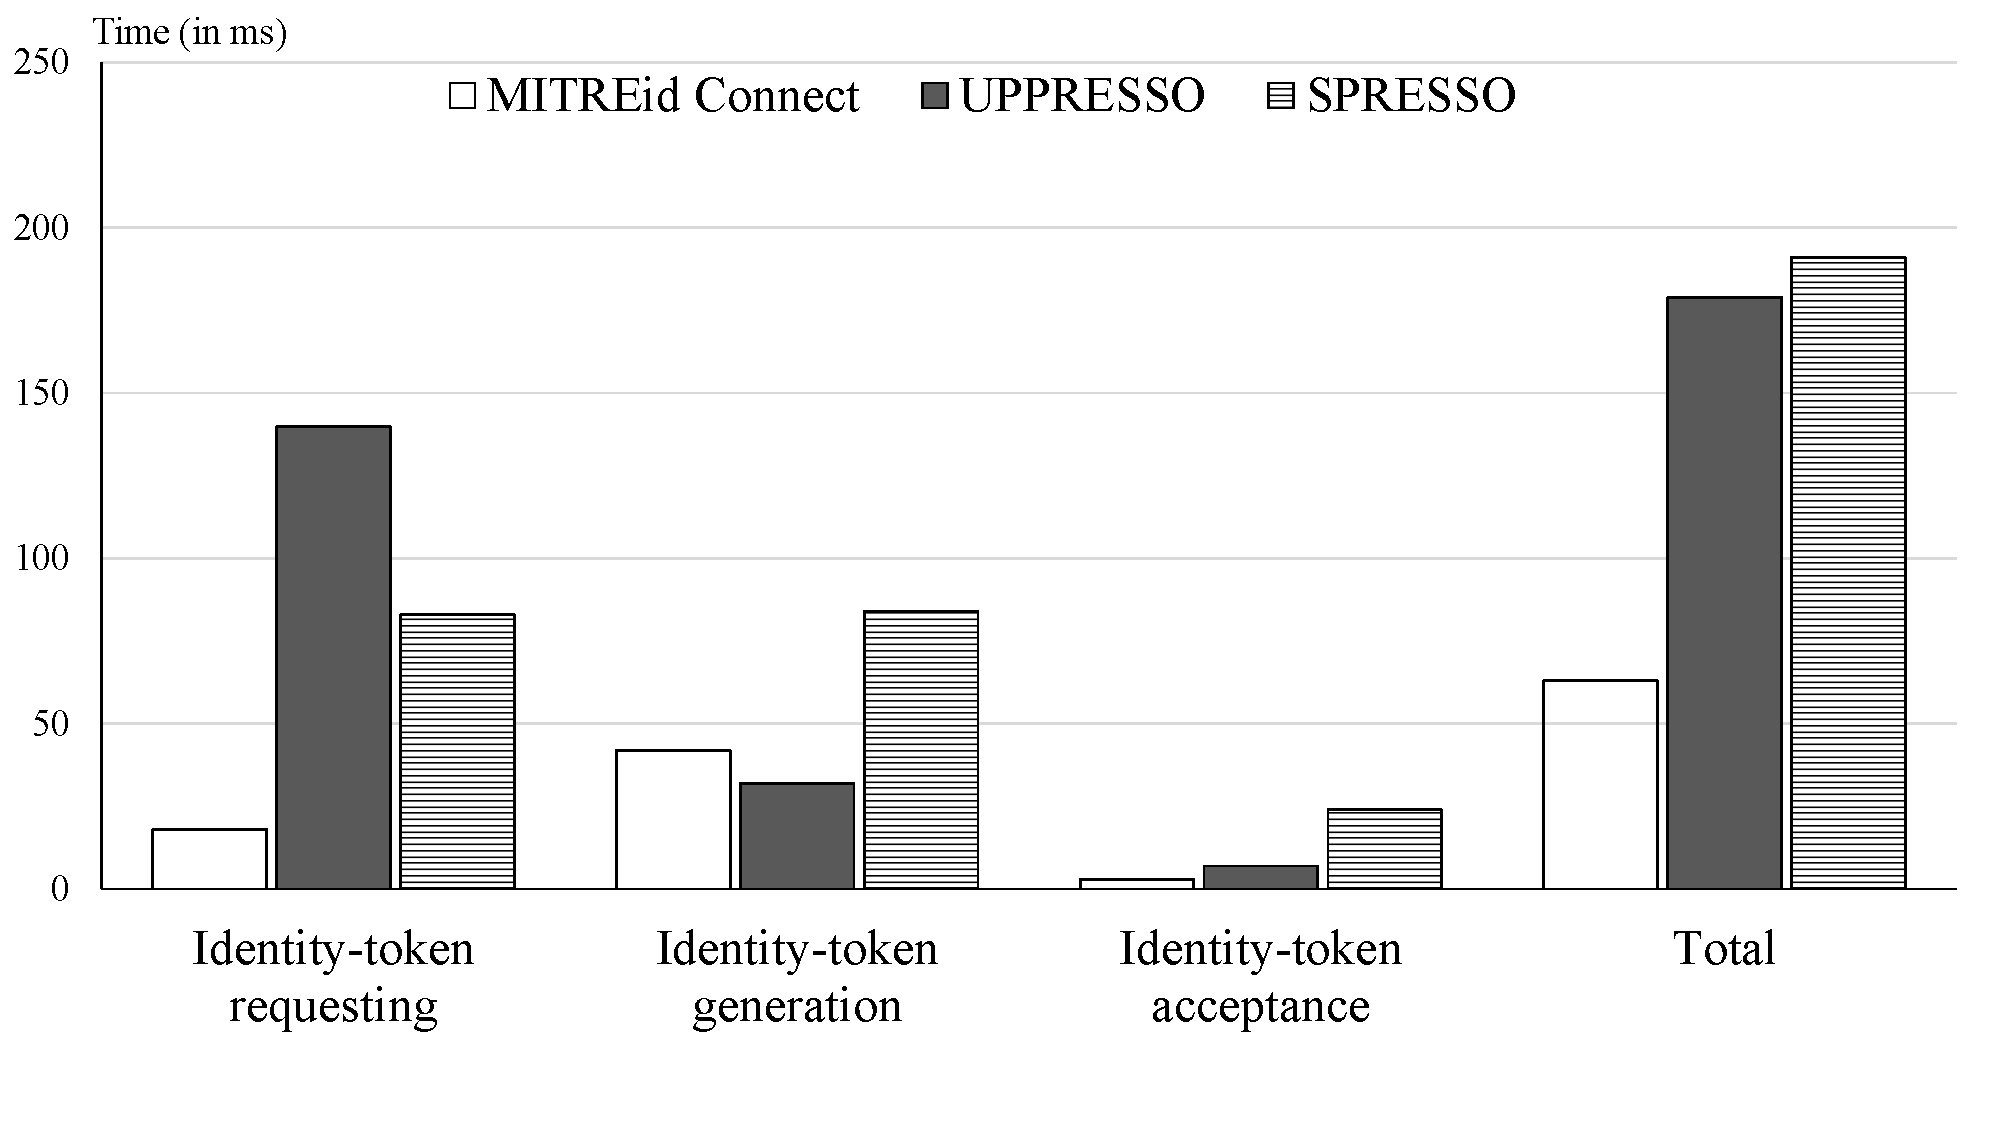
\includegraphics[width=0.97\linewidth]{fig/evaluation-lan.pdf}
		\end{minipage}}
	\subfigure[With a remotely-visiting browser]{
  		\begin{minipage}[b]{0.45\textwidth}
			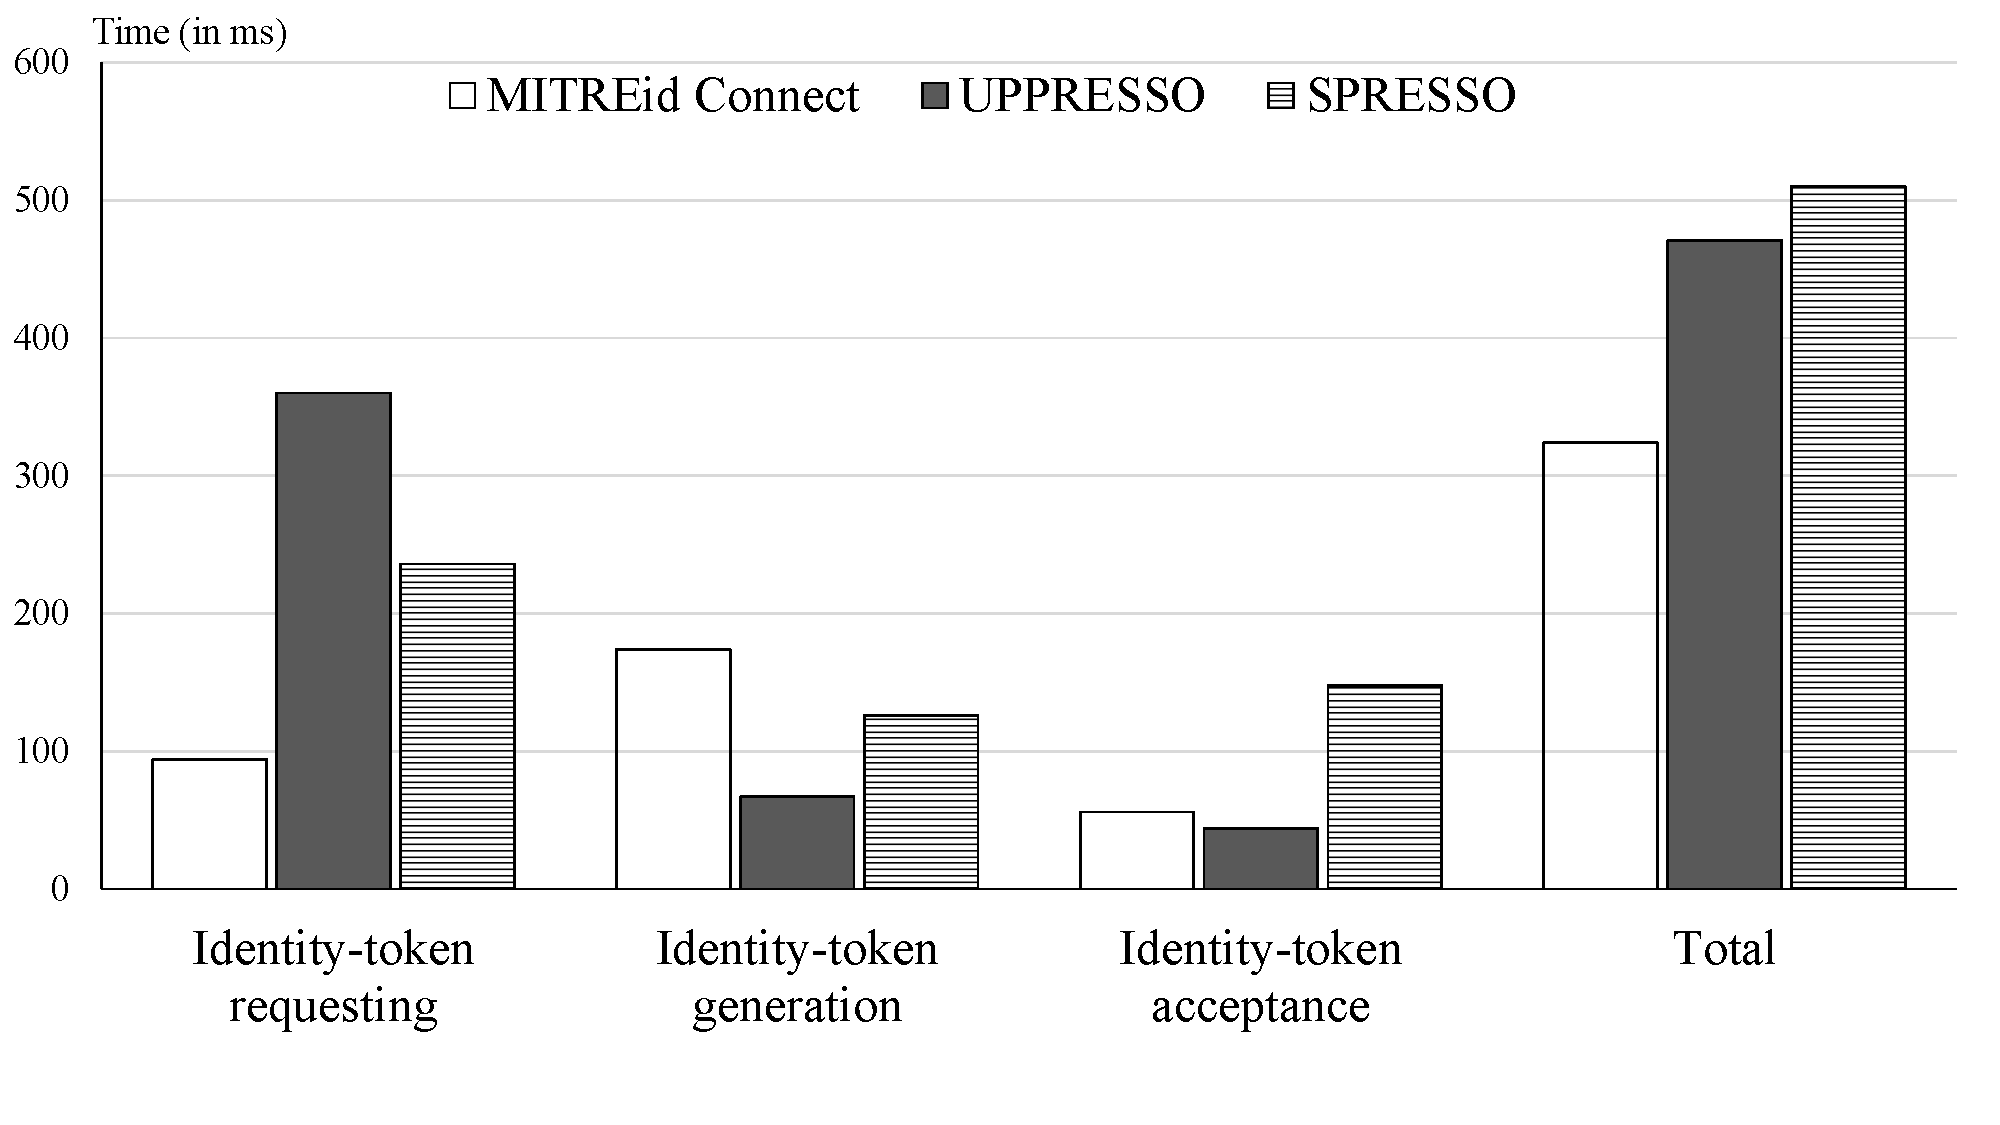
\includegraphics[width=0.97\linewidth]{fig/evaluation-internet.pdf}
		\end{minipage}}
  \caption{The time costs of SSO login in MITREid Connect, UPPRESSO, and SPRESSO}
  \label{fig:evaluation}
\end{figure}

Regarding identity-token requesting, %the user browser loads the RP's webpage and starts the login request.
the RP of MITREid Connect immediately constructs an identity-token request. %MITREid Connect only needs 10 ms but UPPRESSO requires 271 ms.
UPPRESSO incurs overheads in opening a new browser window and downloading the scripts.
%
%\footnote{This pop-up overhead can be reduced %by silently conducting these operations when the user visits the RP website, or
%by browser extensions.
%We have implemented such a browser extension while keeping the IdP and RPs unmodified, and the supplementary experiments showed a reduction of (\emph{a}) about 90 ms in the virtual private cloud setting and (\emph{b}) 260 ms when accessed remotely.}
%
In SPRESSO the RP needs to obtain information about the IdP % 's public key %(SPRESSO allows a user to assign any IdPs before login without initial registrations)
and encrypt its domain using an ephemeral key, resulting in extra overheads.

UPPRESSO requires the least time for generating identity tokens for it receives the token from the IdP without any additional processing.
MITREid Connect and SPRESSO require extra time as the browser downloads a script from the RP in this phase. % to process the token retrieved from the IdP, which is carried with a URL following the fragment identifier \texttt{#} instead of \texttt{?} due to security considerations \cite{de2014oauth}.
Moreover, SPRESSO takes slightly more time to generate an identity token, as it implements the IdP using node.js and uses a JavaScript cryptographic library that is a little less efficient than the Java library used in the others.

In the identity-token acceptance phase, 
MITREid Connect and UPPRESSO take similar amounts of time for the RP to receive a token and accept it.
In contrast, SPRESSO takes the longest time due to its complex processing at the user agent.
After receiving an identity token from the IdP, the browser downloads another script from the forwarder server, to decrypt the RP endpoint and sends the token to this endpoint.

